\section{A reproducible boundary experiment}
\label{sec:experiments}
We evaluate the family in Theorem~\ref{thm:normal_separation} with
$a=0.7$, $\varepsilon=10^{-6}$, $L_{\rm init}=1$, and
$A\in\{0,1,10,100,1000\}$. The comparison uses
\eqref{eq:vyguzov_step} with $L_0=L_1=1$ and the exact-oracle
backtracking rule. Both retain the same lower-bound certificate.
The full box linear oracle uses a fixed tie rule. There is no sampling
or parameter tuning across these ten deterministic runs.

\begin{table}[H]
\centering
\caption{Accepted updates and objective calls. Every backtracking run
uses three gradients and three full linear minimizations.}
\label{tab:boundary}
\begin{tabular}{rrrrr}
\toprule
$A$ & Fixed rule & Backtracking & Fixed $N_f$ & Backtracking $N_f$\\
\midrule
0    & 11   & 2 & 12   & 5\\
1    & 14   & 2 & 15   & 5\\
10   & 66   & 2 & 67   & 5\\
100  & 610  & 2 & 611  & 5\\
1000 & 6045 & 2 & 6046 & 5\\
\bottomrule
\end{tabular}
\end{table}

All runs stop at $(-1,0)$ with zero gap. The backtracking traces agree
exactly across the five values of $A$: the first accepted curvature is
two, the second is one, and there are two rejected trials in total.
At $A=1000$, the gradient norm at the solution is approximately
$1000.000068$, while the objective error and the certificate are zero.

\begin{figure}[H]
\centering
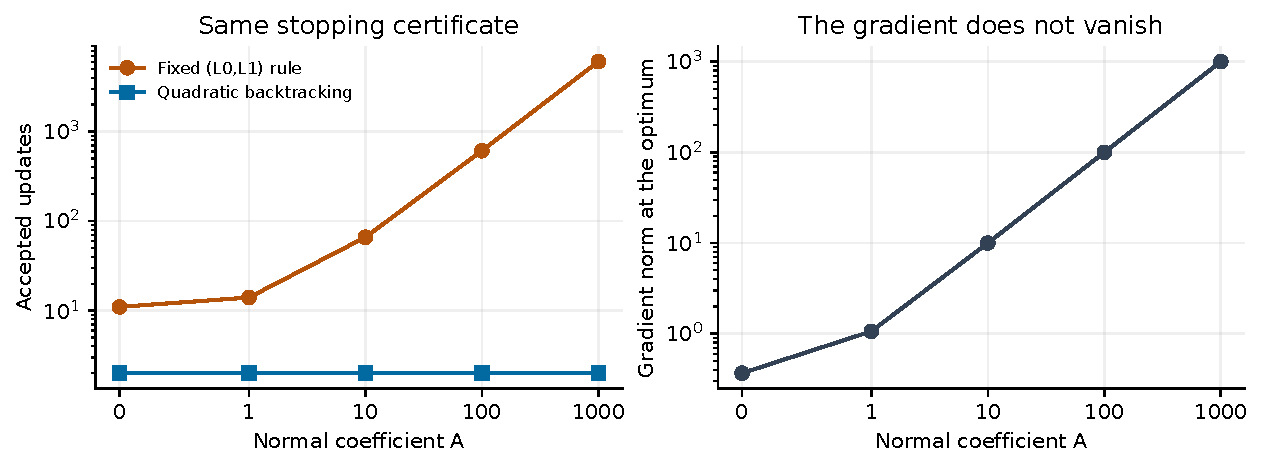
\includegraphics[width=\linewidth]{figures/boundary_normal_benchmark.pdf}
\caption{The fixed norm-based step becomes smaller as the normal
coefficient grows. Backtracking has the same two-update execution,
although the gradient at the minimizer grows without bound.}
\label{fig:boundary}
\end{figure}

The script \texttt{Code/benchmark\_boundary.py} writes every visited
point, gap, retained certificate, accepted curvature, and oracle count.
It checks feasibility, objective decrease, the analytical crossing
bound~\eqref{eq:normal_lower}, and equality of the backtracking traces.
The known solution is used only for a diagnostic after stopping.
The algorithm itself receives neither the minimizer nor its value.
The experiment uses Python floating-point arithmetic; the statements
in Sections~\ref{sec:stopping} and~\ref{sec:normal} are proved
independently of these numerical checks.

\paragraph{Reading the result.}
The full gap resolves the stopping issue at a boundary minimum.
Quadratic backtracking also avoids an unnecessary dependence on the
normal coefficient in the product family of
Proposition~\ref{prop:normal_invariance}. The comparison in
Table~\ref{tab:boundary} uses the fixed Algorithm~1 of~\cite{vyguzov};
the proof and the table make the same comparison.

\paragraph{Use of computational tools.}
AI tools assisted with derivations, checks, implementation, and writing.
The authors are responsible for validating the mathematical claims,
sources, and reported computations.
